\chapter{奇异关联子与全息张量网络}
\label{chap:strange-correlator}

\section{弦网模型基态的张量网络表示}

\subsection{四面体对称性}
\label{subsec:tetrahedral-symmetry}

我们在式~\eqref{eq:f-move} 和 \eqref{eq:string-net-local-rules} 中分别给出了 $F$ 符号的两种定义:
\begin{equation}
  \begin{aligned}
       \tikzinput{category-theory/f-symbol-1}
    &= \sum_y \, \bigl[ F^{abc}_d \bigr]_{xy} \tikzinput{category-theory/f-symbol-2}, \\
       \tikzinput{category-theory/f-symbol-3}
    &= \sum_m F^{ijm}_{kln} \tikzinput{category-theory/f-symbol-4}.
  \end{aligned}
\end{equation}
容易知道 $[F^{ijk}_l]_{xy}=F^{jix}_{lky}$。在本文中我们主要使用第一种定义。另一方面,根据式~\eqref{eq:f-move},我们有
\begin{equation}
    \bigl[ F^{abc}_d \bigr]_{xy}
  = \frac{\tr \, \Biggl[
      \Biggl( \tikzinput{category-theory/f-symbol-small-2} \Biggr)^\dagger \,
      \tikzinput{category-theory/f-symbol-small-1}
    \Biggr]}{\tr \, \Biggl[
      \Biggl( \tikzinput{category-theory/f-symbol-small-2} \Biggr)^\dagger \,
      \tikzinput{category-theory/f-symbol-small-2}
    \Biggr]}
  = \frac{\tikzinput{category-theory/f-symbol-trace-1}}{\tikzinput{category-theory/f-symbol-trace-2}}.
\end{equation}
这里分母部分可以利用环路消除 \eqref{eq:loop-removal} 式化简:
\begin{equation}
  \tikzinput{category-theory/f-symbol-trace-2} = \sqrt{d_a d_b d_c d_d},
\end{equation}
而分子部分则等价于一个正四面体,于是
\begin{equation}
    \bigl[ F^{abc}_d \bigr]_{xy}
  = \sqrt{d_x d_y} \, \begin{bmatrix} a & b & x \\ c & d & y \end{bmatrix}
  = \frac{1}{\sqrt{d_a d_b d_c d_d}} \, \Tetrahedron xbdyca.
\end{equation}
式中
\begin{equation}
    \begin{bmatrix} a & b & c \\ i & j & k \end{bmatrix}
  = \frac{1}{\sqrt{d_a d_b d_c d_i d_j d_k}} \, \Tetrahedron cbjkia
\end{equation}
称为\emph{四面体符号} (tetrahedral symbol),它的对称性(以及相应 $F$ 符号的对称性)可以从四面体的几何性质中获得:
\begin{align}
     \begin{bmatrix} a & b & c \\ i & j & k \end{bmatrix}
  &= \begin{bmatrix} b & c & a \\ j & k & i \end{bmatrix}
   = \begin{bmatrix} c & a & b \\ k & i & j \end{bmatrix}, \\
     \begin{bmatrix} a & b & c \\ i & j & k \end{bmatrix}
  &= \begin{bmatrix} a & c & b \\ i & k & j \end{bmatrix}
   = \begin{bmatrix} c & b & a \\ k & j & i \end{bmatrix}
   = \begin{bmatrix} b & a & c \\ j & i & k \end{bmatrix}, \\
     \begin{bmatrix} a & b & c \\ i & j & k \end{bmatrix}
  &= \begin{bmatrix} a & j & k \\ i & b & c \end{bmatrix}
   = \begin{bmatrix} i & b & k \\ a & j & c \end{bmatrix}
   = \begin{bmatrix} i & j & c \\ a & b & k \end{bmatrix}.
\end{align}
以上三组等式分别对应了四面体对称群 $A_4$ 中绕顶角的旋转(列轮换)、镜像(交换两列)和绕对边连线的旋转(交换两行的部分)。注意整行的交换一般来说并不相等。这一性质为\emph{四面体对称性} (tetrahedral symmetry)\cite{aasen2020topological,fuchs2023tetrahedral}。利用 $F$ 移动和环路消除,还可以得到下面的关系式:
\begin{equation}
    \tikzinput{string-net/vertex-2}
  = \sqrt{d_\alpha d_\beta d_\gamma} \, \begin{bmatrix} a & b & c \\ \alpha & \beta & \gamma \end{bmatrix} \Vertex kij
  = \frac{1}{\sqrt{d_i d_j d_k}} \, \Tetrahedron ik\gamma\alpha\beta j \Vertex kij,
\end{equation}
这也被称为\emph{星—三角变换} (star-triangle transformation)。

\subsection{弦网模型的基态}

接下来我们来给出弦网模型基态的张量网络表示\cite{gu2009tensor2,buerschaper2009explicit}。由于弦网模型的 Hamilton 量
\begin{equation}
  H = -\sum_v A_v - \sum_p B_p
\end{equation}
是严格可解的,即 $H$ 可以表示成一系列相互对易的投影算符之和,因而它的基态可以通过这些投影算符的本征子空间给出。式中,电荷算符 $A_v$ 指定了每个顶点处的融合规则,磁通算符 $B_p$ 是 $B_p^s$ 按量子维数的线性组合,而 $B_p^s$ 则可以图形化地视为能在方块 $p$ 处生成一个孤立环路的算符(具体定义见 \ref{subsec:string-net-hamiltonian} 小节)。

弦网模型的基态波函数 $\ket{\psi_0}$ 可以通过在真空态 $\ket{\varnothing}$ 上作用全部的 $B_p$ 算符得到。如上所言,每个 $B_p$ 算符都是一个方块内部由对象 $R$ 构成的环路,而
\begin{equation}
  \tikzinput{string-net/string-1}
  \enspace = \sum_i \frac{d_i}{D^2}
  \tikzinput{string-net/string-2}
\end{equation}
则是任意子按量子维数的加权叠加。因此有
\begin{equation}
    \ket{\psi_0} = \prod_p B_p \ket{\varnothing}
  = \prod_p B_p \, \ket[\Bigg]{\, \tikzinput{string-net/loop-3} \,}
  = \ket[\Bigg]{\, \tikzinput{string-net/loop-4} \,}.
\end{equation}

为了给出 $\ket{\psi_0}$ 一种\emph{对称化}的张量网络表示,我们必须从一开始就同等对待六边形的每个边以保持对称性。需要指出的是,文献 \parencite{buerschaper2009explicit} 中通过引入奇偶子网格来构造张量网络的手段不能很好地保留旋转对称性。这里,我们需将权重(量子维数)$d_i$ 平均分配到 $R$ 环路的六个边上,使得它们在互相连接时也有良好定义:
\begin{equation}
  \begin{aligned}
       \VirutalHexagon{\draw [very thick, draw=MaterialRed] (-30:0.8) -- (30:0.8)} \enspace
    &= \sum_i \left( \frac{d_i}{D^2} \right)^{1/6} \enspace
       \VirutalHexagon{\draw [thick] (-30:0.8) node [left] {$i$} -- (30:0.8)} \, , \\
       \VirutalHexagon{\draw [very thick, draw=MaterialRed] (-30:0.8) -- (30:0.8) -- (90:0.8)} \enspace
    &= \sum_i \left( \frac{d_i}{D^2} \right)^{1/3} \enspace
       \VirutalHexagon{\draw [thick] (-30:0.8) node [left] {$i$} -- (30:0.8) -- (90:0.8)} \, , \\
       \VirutalHexagon{\draw [very thick, draw=MaterialRed] (0,0) circle [radius=0.7]} \enspace
    &= \sum_i \frac{d_i}{D^2} \enspace
       \VirutalHexagon{\draw [thick] (0,0) circle [radius=0.7] node [right=-0.2em] {$i$}} \, .
  \end{aligned}
\end{equation}
对于邻接的六边形,我们可以在两个相邻的 $R$ 环路间执行 $F$ 移动:
\begin{align}
     \tikzinput{string-net/adjacent-loop-1} \enspace
  &= \sum_{i,j} \biggl( \frac{d_i d_j}{D^4} \biggr)^{1/6} \enspace
     \tikzinput{string-net/adjacent-loop-2} \notag \\
  &= \sum_{i,j} \biggl( \frac{d_i d_j}{D^4} \biggr)^{1/6} \sum_k \sqrt{\frac{d_k}{d_i d_j}} \enspace
     \tikzinput{string-net/f-move-1} \notag \\
  &= \sum_{i,j,k} \bigl( D^2 d_i d_j \bigr)^{-1/6} d_k^{1/4} \cdot \bigl( D^2 d_i d_j \bigr)^{-1/6} d_k^{1/4} \enspace
     \tikzinput{string-net/f-move-1} \,
   = \tikzinput{string-net/f-move-2} \, .
\end{align}
式中,蓝线和紫线表示各任意子按照对应量子维数的加权叠加,并且分别带有 $(D^2 d_i d_j)^{-1/6}$ 和 $d_k^{1/4}$ 的因子。在对所有的 $R$ 环路执行 $F$ 移动之后,$\ket{\psi_0}$ 现在可以表示为
\begin{equation}
  \ket{\psi_0} = \ket[\Bigg]{\, \tikzinput{string-net/vertices}}.
\end{equation}
它可以通过对位于顶点处的局域构建块进行缩并得到,而这些构建块可以用任意子基 (anyon basis) 表示为
\begin{align}
     \tikzinput{string-net/vertex-1} \enspace
  &= \sum_{i,j,k} \sum_{\alpha,\beta,\gamma} D^{-1} (d_i d_j d_k)^{1/4} (d_\alpha d_\beta d_\gamma)^{-1/3} \,
     \tikzinput{string-net/vertex-2} \notag \\
  &= \sum_{i,j,k} \sum_{\alpha,\beta,\gamma} D^{-1} (d_i d_j d_k)^{-1/4} (d_\alpha d_\beta d_\gamma)^{-1/3}
     \Tetrahedron ik\gamma\alpha\beta j \Vertex kij.
\end{align}
这样我们就获得了六边形网格中三角形张量的对称形式:
\begin{align}
  \Triangle jki\alpha\beta\gamma
  &= D^{-1} (d_i d_j d_k)^{-1/4} (d_\alpha d_\beta d_\gamma)^{-1/3} \,
    \Tetrahedron ik\gamma\alpha\beta j \notag \\
  &= D^{-1} (d_\alpha d_\beta d_\gamma)^{1/6} (d_i d_j d_k)^{-1/4} (d_\alpha d_\beta d_\gamma)^{-1/2} \,
    \Tetrahedron ik\gamma\alpha\beta j.
  \label{eq:unit-of-string-net-honeycomb}
\end{align}
对于更一般的情形,因子 $1/6$ 需要根据闭合环路中每条边的贡献进行修正。在任意三价图(每个顶点与三条边相连)中,归一化的三角形张量可以写成
\begin{align}
  \Triangle jki\alpha\beta\gamma
  &= D^{-2 (1/n_\alpha + 1/n_\beta + 1/n_\gamma)}
    \bigl( d_\alpha^{1/n_\alpha} d_\beta^{1/n_\beta} d_\gamma^{1/n_\gamma} \bigr) \notag \\
  &\qquad \cdot (d_i d_j d_k)^{-\frac14} (d_\alpha d_\beta d_\gamma)^{-\frac12} \,
    \Tetrahedron ik\gamma\alpha\beta j,
  \label{eq:unit-of-string-net-general}
\end{align}
这些三角形张量每条边带有三个指标,外面的两个是\emph{虚拟指标}或\emph{辅助指标},它们会在平面内互相缩并掉;中间的一个则是\emph{物理指标},它们会伸出平面外,并且不会被缩并掉。可以看出,这实际上也是一种 PEPS 张量网络(见 \ref{subsec:mps-generalization} 小节)。

\begin{figure}[htb]
  \centering
  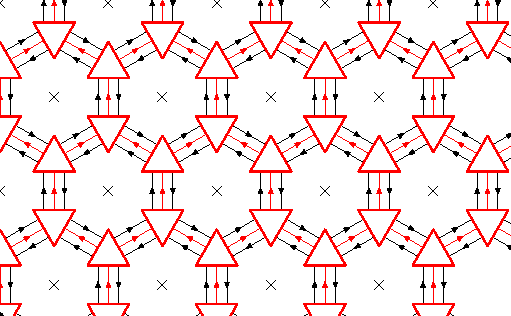
\includegraphics[width=0.6\textwidth]{images/temp/string-net-peps.pdf}
  \caption[弦网模型基态的 PEPS 张量网络表示]{弦网模型基态的 PEPS 张量网络表示。图片来源:\parencite{buerschaper2009explicit}。}
  \label{fig:string-net-peps}
\end{figure}

\section{奇异关联子}
\label{sec:strange-correlator}

\emph{奇异关联子} (strange correlator) 最早用来在对称保护拓扑序 (symmetry protected topological order, SPT)\footnote{尽管名称中带有“拓扑序”,但 SPT 态中只有短程纠缠,这与本文所说的拓扑序(具有长程纠缠,见 \ref{sec:topological-order} 节)实际上是不同的。} 中寻找不同的相\cite{you2014wave},之后则被推广到了弦网模型中\cite{vanhove2018mapping,lootens2019cardy,vanhove2022topological}。通过将 2+1 维弦网模型的 PEPS 基态波函数 $\ket{\Psi_\text{SN}}$ 与某些特定的直积态 $\ket{\Omega}$ 做内积,可以获得二维临界格点模型的配分函数
\begin{equation}
  Z = \langle\Omega|\Psi_\text{SN}\rangle.
\end{equation}
在热力学极限下,配分函数 $Z$ 可由对应的共形场论 (CFT) 来描述。如图~\ref{fig:peps-strange-correlator} 所示,对于由三角形张量单元构成的 PEPS 张量网络,直积态 $\ket{\Omega}$ 相当于为其提供了特定的边界条件,即把物理指标固定到某些值上,而角落上的自由度则需求和。

\begin{figure}[htb]
  \centering
  \tikzinput{strange-correlator}
  \caption[奇异关联子]{奇异关联子。其中绿线表示投影到特定值(即与某直积态做内积)之后的物理指标,灰线表示需要求和的辅助指标。整个张量网络缩并后即为对应的配分函数。}
  \label{fig:peps-strange-correlator}
\end{figure}

\subsection{例子:Fibonacci 模型}
\label{subsec:strange-correlator-fib}

接下来,我们利用 \ref{subsec:fusion-category-examples} 小节中所给出的 Fibonacci 和 Ising 两种融合范畴的数据来构造相应的奇异关联子。Fibonacci 弦网模型定义在六边形网格上,它包含 $\1$ 和 $\tau$ 两种简单对象(任意子),量子维数分别为 $d_{\1}=1$、$d_\tau=\varphi$,其中 $\varphi=(1+\sqrt5)/2$ 是黄金比。融合规则为
\begin{equation}
  \1 \times \1 = \1, \quad
  \1 \times \tau = \tau \times \1 = \tau, \quad
  \tau \times \tau = \1 + \tau,
\end{equation}
$F$ 符号为
\begin{equation}
  [F^{\tau\tau\tau}_\tau]_{ij} = \dfrac1\varphi \begin{pmatrix} 1 & \sqrt\varphi \\ \sqrt\varphi & -1 \end{pmatrix}, \quad
  i,j \in \{\1, \tau\}.
\end{equation}
唯一非平凡的四面体以及对应的三角形张量为
\begin{equation}
  \begin{aligned}
       \Tetrahedron \tau mn\tau\tau\tau
    &= \sqrt{d_\tau d_\tau d_\tau d_\tau} \bigl[ F^{\tau\tau\tau}_\tau \bigr]_{mn}
     = \varphi^2 \bigl[ F^{\tau\tau\tau}_\tau \bigr]_{mn}, \\
       \Triangle \tau\tau mn\tau\tau
    &= (d_\tau d_\tau d_m)^{-\frac14} (d_\tau d_\tau d_n)^{-\frac13} \Tetrahedron \tau mn\tau\tau\tau \\
    &= \varphi^{\frac56} d_m^{-\frac14} d_n^{-\frac13} \bigl[ F^{\tau\tau\tau}_\tau \bigr]_{mn}, \enspace
       m,n \in \{\1,\tau\}.
  \end{aligned}
\end{equation}
在我们的奇异关联子构造中,所有的物理指标都会被选取为 $\tau$,因而这时将得到两种三角形张量单元:
\begin{equation}
    \Triangle \tau\tau\tau\tau\tau\tau
  = \varphi^{\frac14} \bigl[ F^{\tau\tau\tau}_\tau \bigr]_{\tau\tau} = -\varphi^{-\frac34}, \quad
    \Triangle \tau\tau\tau\1\tau\tau
  = \varphi^{\frac{7}{12}} \bigl[ F^{\tau\tau\tau}_\tau \bigr]_{\tau\1} = \varphi^{\frac{1}{12}}.
\end{equation}

\subsection{例子:Ising 模型}

为了与经典二维 Ising 模型相对应,我们考虑一个定义在正方形和八边形交错的网格上、由 $\1$、$\sigma$ 和 $\psi$ 三种简单对象构成的 Ising 弦网模型。各任意子对应的量子维数分别为 $d_{\1}=d_\psi=1$、$d_\sigma=\sqrt2$,融合规则为
\begin{equation}
  \begin{gathered}
  \1 \times \1 = \psi \times \psi = \1, \quad
  \1 \times \sigma = \sigma \times \1 = \sigma \times \psi = \psi \times \sigma = \sigma, \\
  \1 \times \psi = \psi \times \1 = \psi, \quad
  \sigma \times \sigma = \1 + \psi,
  \end{gathered}
\end{equation}
$F$ 符号为
\begin{equation}
  [F^{\psi\sigma\psi}_\sigma]_{\sigma\sigma} = [F^{\sigma\psi\sigma}_\psi]_{\sigma\sigma} = -1, \quad
  [F^{\sigma\sigma\sigma}_\sigma]_{ij} = -\dfrac{1}{\sqrt2} \begin{pmatrix} 1 & 1 \\ 1 & -1 \end{pmatrix}, \quad
  i,j \in \{\1, \psi\}.
\end{equation}
于是四面体和三角形张量为:
\begin{equation}
  \begin{aligned}
       \Triangle \sigma\sigma\1\1\sigma\sigma
    &= (d_{\1} d_\sigma d_\sigma)  ^{-\frac14} (d_{\1} d_\sigma d_\sigma)  ^{-\frac13}
       \Tetrahedron \1\sigma\sigma\1\sigma\sigma
       = 2^{-\frac{1}{12}}, \\
       \Triangle \sigma\sigma\1\psi\sigma\sigma
    &= (d_{\1} d_\sigma d_\sigma)  ^{-\frac14} (d_\sigma d_\sigma d_\psi)^{-\frac13}
       \Tetrahedron \1\sigma\sigma\psi\sigma\sigma
       = 2^{-\frac{1}{12}}, \\
       \Triangle \sigma\sigma\psi\1\sigma\sigma
    &= (d_\sigma d_\sigma d_\psi)^{-\frac14} (d_{\1} d_\sigma d_\sigma)  ^{-\frac13}
       \Tetrahedron \psi\sigma\sigma\1\sigma\sigma
       = 2^{-\frac{1}{12}}, \\
       \Triangle \sigma\sigma\psi\psi\sigma\sigma
    &= (d_\sigma d_\sigma d_\psi)^{-\frac14} (d_\sigma d_\sigma d_\psi)^{-\frac13}
       \Tetrahedron \psi\sigma\sigma\psi\sigma\sigma
       = -2^{-\frac{1}{12}}.
  \end{aligned}
\end{equation}
在 Ising 模型的奇异关联子构造中,我们需要将物理指标投影到直积态
\begin{equation}
  \bra{\omega(\beta)} = \sqrt2 \, \bigl( \cosh\beta \bra{\1} + \sinh\beta \bra{\psi} \bigr)
\end{equation}
上面。为了得到正方形网格的结构,我们用 8 个三角形组成一个带有 4 个指标的八边形张量单元:
\begin{equation}
  A_{ijkl} = \tikzinput{ising/octagon} \quad \text{where} \quad
  i, j, k, l = \1 \text{ or } \psi, \quad
  \tikzinput{ising/line-sigma} \, = \sigma, \quad
  \tikzinput{ising/line-omega} \, = \omega.
  \label{eq:ising-octagon}
\end{equation}
注意此时物理指标已被求和,而辅助指标 $i$、$j$、$k$、$l$ 得以保留。为了得到 $A_{ijkl}$ 的值,我们先计算每一对三角形:
\begin{equation}
  \tikzinput{ising/triangles-1} = \tikzinput{ising/triangles-2} =
  \begin{cases}
    2^{\frac13} \bigl( \cosh\beta + \sinh\beta \bigr) = 2^{\frac13} \ee^\beta,
      & (i,j) = (\1,\1) \text{ or } (\psi, \psi); \\
    2^{\frac13} \bigl( \cosh\beta - \sinh\beta \bigr) = 2^{\frac13} \ee^{-\beta},
      & (i,j) = (\1,\psi) \text{ or } (\1, \psi).
  \end{cases}
\end{equation}
于是
\begin{equation}
  A_{\1\1\1\1} = A_{\psi\psi\psi\psi} = 2^{\frac43} \ee^{4\beta}, \quad
  A_{\1\psi\1\psi} = A_{\psi\1\psi\1} = 2^{\frac43} \ee^{-4\beta}, \quad
  \text{others} = 2^{\frac43}.
  \label{eq:ising-tensor-from-sc}
\end{equation}
这和围绕一个方块的 Ising 相互作用(4 个自旋)的张量表示 \eqref{eq:ising-tensor} 是一致的,只相差一个整体因子:
\begin{equation}
  A_{ijkl}
    := A_{\sigma_i \sigma_j \sigma_k \sigma_l}
    = \ee^{\beta(\sigma_i\sigma_j + \sigma_j\sigma_k + \sigma_k\sigma_l + \sigma_l\sigma_i)},
  \label{eq:ising-tensor}
\end{equation}

% TODO: dual lattice
把这些八边形张量移动 $1/2$ 格可以获得对偶网格的张量表示
\begin{equation}
  \tilde{A}_{ijkl} = \, \tikzinput{ising/dual-octagon} \quad \text{where} \quad
  i, j, k, l = \1 \text{ or } \psi.
\end{equation}
此时
\begin{equation}
  \tikzinput{ising/dual-triangles-1} = \tikzinput{ising/dual-triangles-2} =
  \begin{cases}
    2^{\frac13} \bigl( \cosh\beta + \sinh\beta \bigr) = 2^{\frac13} \ee^\beta,
      & (i,j) = (\1,\1) \text{ or } (\psi, \psi); \\
    2^{\frac13} \bigl( \cosh\beta - \sinh\beta \bigr) = 2^{\frac13} \ee^{-\beta},
      & (i,j) = (\1,\psi) \text{ or } (\1, \psi).
  \end{cases}
\end{equation}
利用 Kramers--Wannier 对偶,即令 $A=\tilde{A}$,就可以得到临界温度
\begin{equation}
  \ee^{2\beta_{\text{c}}} = \sqrt{2} + 1 \implies \beta_{\text{c}} = \frac12 \log(1 + \sqrt{2}).
\end{equation}

\subsection{中心荷的计算}
\label{subsec:central-charge}

得到奇异关联子后,我们可以用标准的张量网络方法对其进行分析。例如,我们可以利用在 \ref{subsec:mps-time-evolution} 小节中介绍的 iTEBD 算法来计算中心荷,其基本思路是:

\begin{enumerate}
  \item 利用奇异关联子构造正方形张量单元 $A_{ijkl}$。在 Ising 的情况中,我们已经得到了这样的表示[式~\eqref{eq:ising-octagon}];而对于 Fibonacci 模型,我们需要把两个三角张量形拼合成一个正方形:
    \begin{equation}
      A_{ijkl} = \tikzinput{fib/square-1}.
    \end{equation}
  \item 按照 iTEBD 算法,用 $A_{ijkl}$ 作为 iMPO 对随机的初始态进行演化,得到正则化的不动点 iMPS $\{\Gamma,\lambda\}$。
  \item 注意 $\lambda$ 是一个对角矩阵,其对角元可用来计算关联长度 $\xi$ 和 von Neumann 纠缠熵 $S_A$:
    \begin{equation}
      \xi = -\frac{1}{\log|\lambda_2 / \lambda_1|}, \quad
      S_A = \sum_i \lambda_i^2 \log \lambda_i^2
    \end{equation}
  \item 利用关联长度与纠缠熵之间满足的关系式
    \begin{equation}
      S_A \sim \frac{c}{6} \log \xi,
    \end{equation}
    可以对使用不同的连接维数 $\chi$ 所获得的数据进行拟合,即可得到中心荷 $c$。
\end{enumerate}

\begin{figure}[htb]
  % TODO: update image
  \centering
  \begin{tabular}{cc}
    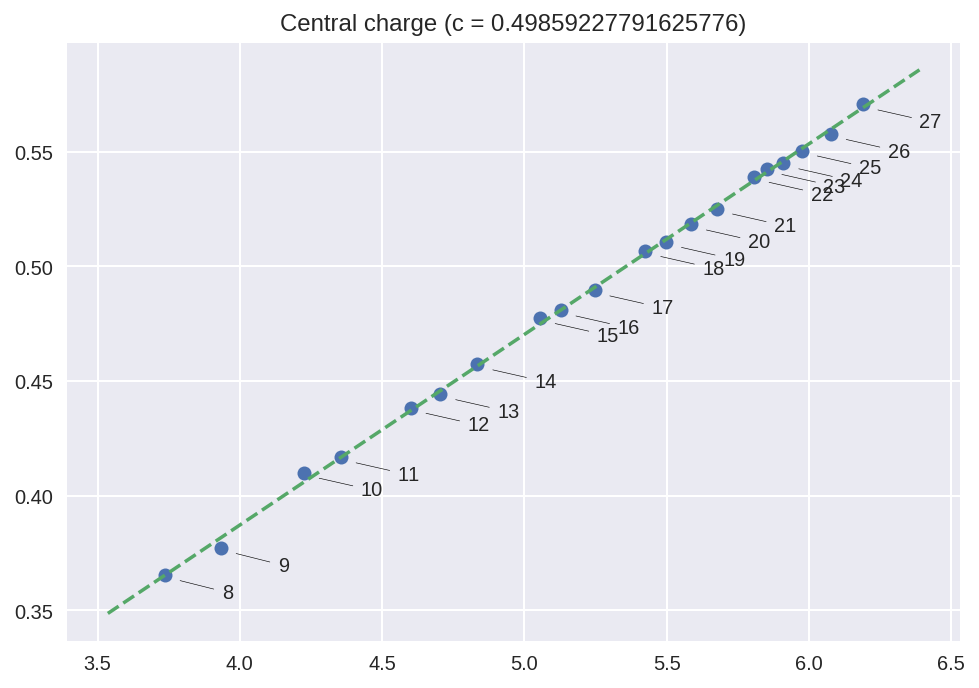
\includegraphics[width=0.45\textwidth]{images/temp/ising-central-charge.png} &
    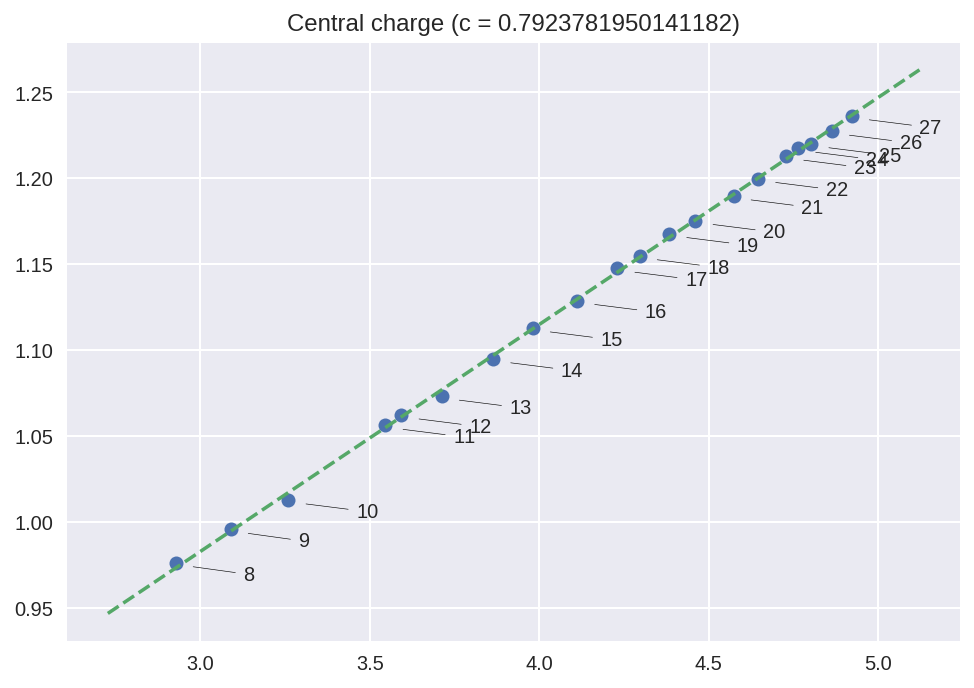
\includegraphics[width=0.45\textwidth]{images/temp/fib-central-charge.png} \\
    (a) Ising 模型 & (b) Fibonacci 模型
  \end{tabular}
  \caption[中心荷拟合结果]{中心荷拟合结果。横坐标:关联长度的对数 $\log\xi$,纵坐标:纠缠熵 $S_A$。使用的连接维数为 $\chi\in\{8,9,\dots,27\}$。}
  \label{fig:central-charge}
\end{figure}

我们使用连接维数 $\chi\in\{8,9,\dots,27\}$ 来进行计算,拟合结果如图~\ref{fig:central-charge} 所示。得到的中心荷为
\begin{equation}
  c_{\text{Ising}} \simeq 0.499 \pm 0.004, \quad
  c_{\text{Fib}}   \simeq 0.792 \pm 0.004.
\end{equation}
这与对应 CFT 给出的理论值 $1/2$ 和 $4/5$ 是非常接近的,说明通过奇异关联子的确可以从弦网模型基态波函数出发得到正确的 CFT 不动点张量。

\subsection{高度模型}

% TODO: height model
\emph{高度模型} (height model)

\section{MPO 对称性}

在弦网模型的 PEPS 张量网络表示中,弦激发可以理解为由满足\emph{推拉条件} (pulling-through condition) 的矩阵乘积算符 (MPO) 产生。这些 MPO 具有一定的代数结构,它们之间满足融合规则:
\begin{equation}
  \text{MPO}_a \, \text{MPO}_b = \sum_c N_{ab}^c \, \text{MPO}_c,
\end{equation}
其中 $N_{ab}^c$ 和输入范畴所给出的数据是一致的。任意子则可通过在 MPO 两端放置缺陷张量来产生,这些 MPO 的对称性给出了另外的 $C^*$ 代数结构,其\emph{中心幂等元} (central idempotent) 也对应了输出范畴的不同\emph{拓扑分区} (topological sector),即不同的任意子类型。

\section{例子}
